\section{方法} 
\label{sec:proposed}

这一章节将对统计方法的纹理分析和基于聚类技术的纹理分割进行介绍,其中本文对统计方法的纹理分析采用了灰度共生矩阵和 Gabor 滤波器两种纹理特征表示方法,其对分割结果将在实验部分给出。

\subsection{纹理表示}

\subsubsection{灰度共生矩阵}

灰度共生矩阵(GLCM, Gray Level Coocurrence Matrices)是描述具有某种空间位置关系两个像素灰度的联合分布概率,不仅反映灰度的分布特性,也反映具有同样灰度或相近灰度的像素之间的位置分布特性,是有关图象灰度变化的二阶统计特征。这是由于纹理是由灰度分布在空间位置上反复出现而形成的,因而在图像空间中相隔某距离的两像素之间会存在一定的灰度关系,即图像中灰度的空间相关特性。灰度共生矩阵描述的从来不是单个像素,而是成对的像素之间的关系,对应的,灰度直方图则可以看做是对单个像素的统计与描述,并不涉及灰度间的关联关系。灰度共生矩阵能反映图像灰度关于方向、相邻间隔、变化幅度等综合信息,它是分析图像的局部模式和它们排列规则的基础。其计算公式定义为:

\begin{equation}
\begin{gathered}
P(i, j \mid \Delta x, \Delta y)=W \cdot Q(i, j \mid \Delta x, \Delta y) \\
W=\frac{1}{(M-\Delta x)(N-\Delta y)}, Q(i, j \mid \Delta x, \Delta y)=\sum_{n=1}^{N-\Delta y} \sum_{m=1}^{M-\Delta x} A \\
A=\left\{\begin{array}{cc}
1 \quad \text { if } \quad f(m, n)=i \text { and } f(m+\Delta x, y+\Delta y)=j \\
0 \text { else }
\end{array}\right.
\end{gathered}
\vspace{0.5cm}
\end{equation}

其中,$P(i,j)$ 为灰度共生矩阵中的元素,表示对于一个有着 $G$ 个灰度级、大小为 $M \times N$的图像而言,沿着图像的某一方向移动距离 $d$,像素的灰度级从 $i$ 变为 $j$ 的概率,$P(i, j \mid \Delta x, \Delta y)$ 也可以用符号 $P(i, j \mid d, \theta)$ 来表示;$f(m,n)$ 表示图像中坐标为 $(m,n)$ 的像素的灰度值。

如图 \ref{fig:glcm_figure} 所示,$x$ 方向是图像的列,$y$ 方向是图像的行,$f(x, y) = i$,为坐标 $(x, y)$ 处的灰度值,灰度共生矩阵需要统计的是距离 $(dx, dy)$ 处 $f(x + dx, y + dy) = j$ 的频数(概率),由于 $(dx, dy)$ 的选择不同,则会导致角度的不同,通常选择 $0°$、$45°$、$90°$ 和 $135°$。

\begin{figure}[!htbp]
	\centering
	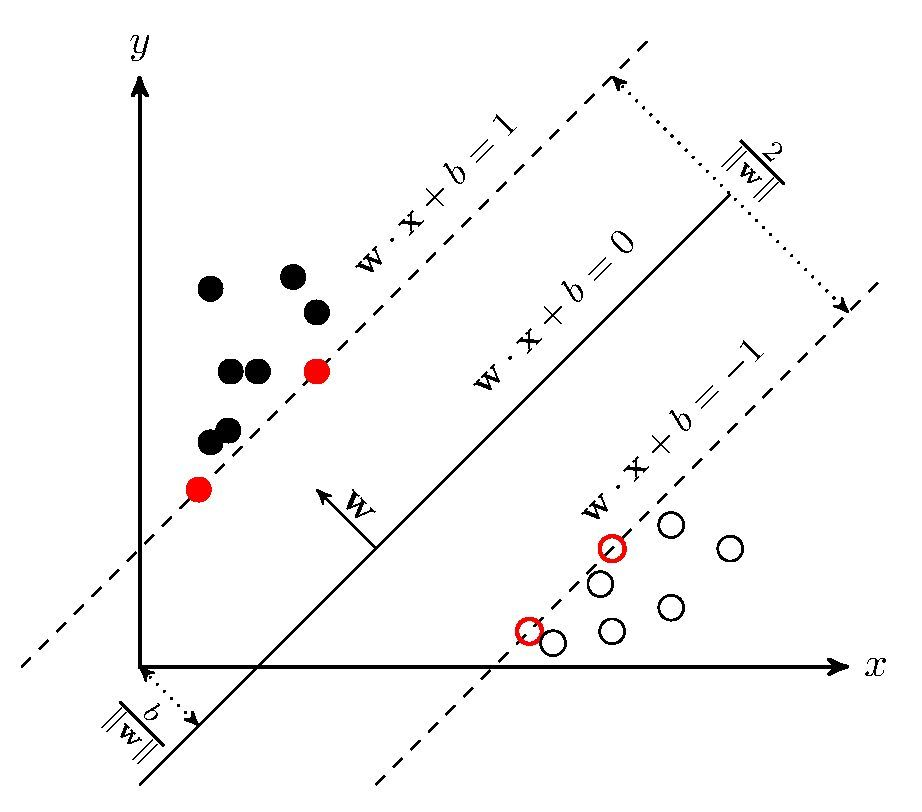
\includegraphics[width=\linewidth]{fig2}
	\caption{灰度共生矩阵的几何表示}
	\label{fig:glcm_figure}
	 \vspace{-0.5cm}
\end{figure}


灰度共生矩阵的计算量是由图像的灰度级和图像的大小共同决定的。例如,假定图像 $I$ 有 $L$ 个灰度级,其大小为 $R \times C$,则运算量大约为 $L^2 \times R \times C$。实际生活中,$L$一般为 $256$, 若令 $R=512, C=512$,则至少要 $1.7 \times 10^{10}$ 次运算,约需耗费30分钟,这显然不太切合实际的。因此在计算灰度共生矩阵时,在不影响纹理特征的前提下往往先对灰度图像的灰度值进行量化,压缩到一个较小的范围,一般取16级。代码实现如下:

\vspace{0.3cm}
\lstinputlisting[language=Python,firstline=35,lastline=41]{main.py}

除此之外,通过直方图均衡化对图像进行预处理也是计算灰度共生矩阵的常用技巧,从而可以消除绝对灰度值的影响。通常,更多地是使用各向同性的灰度共生矩阵来提取具有旋转不变性的纹理特征,即分别计算 $0°$、$45°$、$90°$ 和 $135°$ 四个方向的灰度共生矩阵,如图 \ref{fig:glcm_sample} 所示,然后求均值得到各向同性的灰度共生矩阵。

\begin{figure}[!htbp]
	\centering
	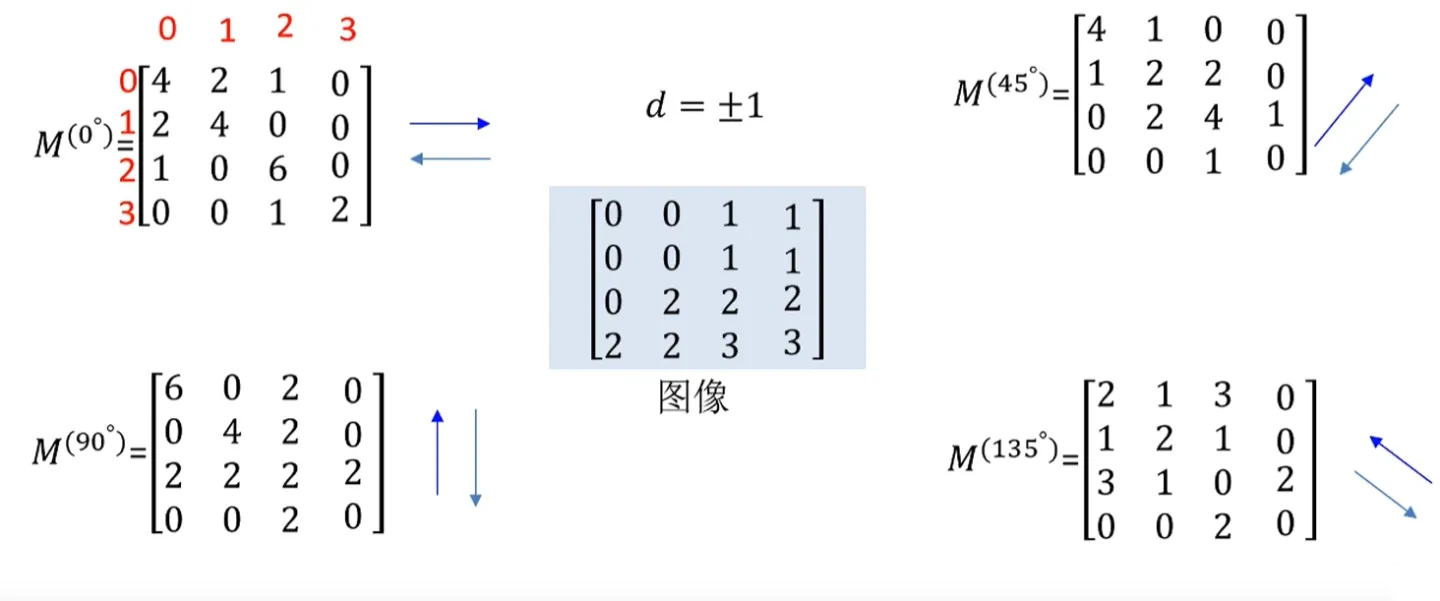
\includegraphics[width=\linewidth]{fig3}
	\caption{简单的图像矩阵及其灰度共生矩阵的示例}
	\label{fig:glcm_sample}
%	 \vspace{-0.5cm}
\end{figure}

统计方法的纹理分析都是通过统计向量(特征向量)来描述区域中的纹理,即在一个局部窗口中计算局部的纹理表征,然后在图像中滑动窗口,最终获得整个图像的纹理表征。灰度共生矩阵也是在这样一个 $w \times w$ 大小的滑动窗口中进行计算的。对于有 $G$ 个灰度级的图像而言,其灰度共生矩阵的维度为 $G \times G$。以图 \ref{fig:glcm_sample} 为例,灰度共生矩阵的计算过程如下:

\begin{enumerate}
	\item 如图 \ref{fig:glcm_sample} 所示,图像的灰度级为4,因此首先创建一个大小为 $4 \times 4$ 的空灰度共生矩阵;
	\item 分别按照 $(d = 1,θ = 0°)$ 、 $(d = 1,θ = 45°)$ 、 $(d = 1,θ = 90°)$ 和 $(d = 1,θ = 135°)$ 进行计算;
	\item 以 $(d = 1,θ = 0°)$ 为例,如第一个值,代表的是图像中灰度值为0,且其水平方向上距离一个像素的点灰度值也为0,即灰度值对 $(0, 0)$ 出现的次数;
	\item 滑动窗口遍历整个图像,并求均值即可完成灰度共生矩阵的计算。
\end{enumerate}

代码实现如下\footnote{由于篇幅原因,部分中间过程代码在此省略}:
\vspace{0.3cm}
\lstinputlisting[language=Python,firstline=118,lastline=135]{main.py}

灰度共生矩阵主要用于纹理特征的提取,但是,一般不直接采用灰度共生矩阵来进行对纹理的统计特性进行度量,而是进一步基于灰度共生矩阵构建统计量。Haralick 提出了14种基于灰度共生矩阵计算出来的统计量,即能量、熵、对比度、均匀性、相关性、方差、和平均、和方差、和熵、差方差、差平均、差熵、相关信息测度以及最大相关系数\footnote{相关统计量的计算方法将在附录 A 给出}。这些特征彼此之间具有较强的相关性,一般采用对比度、角度方向二阶矩、熵和平均值来描述纹理的特性。本文采用了如表 \ref{tab:measurement} 所示的统计量,在将统计量可视化的基础上针对不同的图像进行选择,尽可能建立最有助于纹理分割的纹理特征表示。部分代码实现如下\footnote{完整代码见附录 B}。

在获得基于灰度共生矩阵的统计量后,对其进行均值滤波和标准化处理可以获得更好的分割效果。

\vspace{0.3cm}
\lstinputlisting[language=Python,firstline=4,lastline=45]{glcm_features.py}

\subsubsection{Gabor 滤波器}

对于纹理分析而言,采用 Gabor 滤波具有较好的时-频局部话特性,它能够同时表示和捕捉二维信号在空间位置、空间频率、方向选择性和相位、频率带宽等方面的信息。用 Gabor 滤波器对图像信号滤波,相当于将其按不同方向、频段进行分解,如果计算经不同方向、频段滤波后的纹理特征,这些特征将具有明显的差异,根据这些差异就可以区分不同的纹理。在计算机视觉和图像处理中,多通道 Gabor 方法被认为是一种非常有用的工具,特别是在纹理分析方面。自从一维 Gabor 函数提出之后,很多学者对 Gabor 分析方法进行了研究,研究表明在哺乳类生物视觉系统中,特别是涉及到纹理方面,Gabor 线性空间滤波器有着非常重要的作用。本文采用的基于 Gabor 滤波器的纹理分析方法\footnote{本方法利用网络资源进行实现,由于篇幅原因其实现不再具体展示}如图 \ref{fig:gabor} 所示。

\begin{figure}[!htbp]
	\centering
	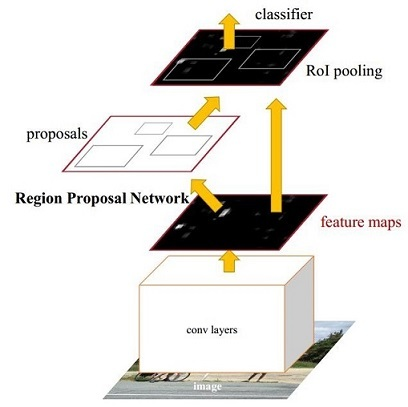
\includegraphics[width=\linewidth]{fig4}
	\caption{基于 Gabor 滤波器的纹理分析及纹理分割算法流程图}
	\label{fig:gabor}
%	 \vspace{-0.5cm}
\end{figure}

Gabor 滤波的方法实际上是多分辨率分解的过程,该方法类似小分析方法。用 Gabor 滤波器进行纹理分析有几个步骤:

\begin{enumerate}
	\item 设计一个对应于不同空间频率和方向的滤波器组;
	\item 把原图像分解为多个滤波图像;
	\item 利用 Gabor 能量特征从滤波图像中提取纹理特征;
	\item 在特征空间中聚类,生成分割图像。
\end{enumerate}

在滤波图像的基础上提取纹理特征,生成特征图像,相同特征区域中的像素具有相同的纹理特性,在特征空间中它们彼此靠近,无监督纹理分割方法即将图像像素聚类到几个簇中,并表现出缘由图像纹理区域,然后给每个簇定义新的标签实现纹理图像分割的目的。一个好的“分类器”在特征空间要实现类内距离尽量小,而类间距离尽量大。下一小节将对基于聚类技术的纹理分割进行介绍。

\subsection{纹理分割}

纹理分割本质上是一个图像分割问题,即采用聚类的方法对图像进行分割,而聚类的特征空间则是由图像的纹理特征构建的。常用的聚类方法,包括 K-Means、Mean-Shift 和 DBScan 等。相较于后者而言,K-Means 更适合本文的实验数据且收敛速度更快,因此,本文将主要对 K-Means 算法进行介绍。 K-Means 算法伪代码如下:
 
 \begin{algorithm}
        \caption{K-Means}
        \LinesNumbered
        \KwIn{输入样本集$D$ = \{$x_1,x_2,\cdots,x_N$\},分簇数$K=n$,最大迭代次数为$M$,从分簇样本中随机选取$n$点\{$u_1$,$u_2,\cdots,u_n$\}作为初始质心}
        \KwOut{输出各样本所在簇\{$C_1$,$C_2$,$\cdots$,$C_n$\}}
        
        \For(\tcp*[f]{$m$表示迭代次数}){$m = 1 \to M$} 
        {
        $C_1 \Leftarrow \emptyset, C_2 \Leftarrow \emptyset,\cdots,  C_n \Leftarrow \emptyset$\tcp*[f]{初始化各簇}
        
            \For(\tcp*[f]{$i$表示样本集编号}){$i = 1,2,...,N$ }     
            {
              $d_{i1} \Leftarrow {\Vert x_i-u_1 \Vert}^2$, $d_{i2} \Leftarrow {\Vert x_i-u_2 \Vert}^2$, $\cdots$, $d_{in} \Leftarrow {\Vert x_i-u_n \Vert}^2$ \tcp*[f]{计算$x_i$到各质心的欧式距离}
              
            \If {$argmin(d_{in}) == n$}
            { $C_n \Leftarrow C_n \cup \{x_i\}$ \tcp*[f]{将$x_i$划分到相应的簇}
            }
            }
            
             $\tilde{u_1} \Leftarrow \frac{1}{\vert C_1 \vert}\sum\limits_{x \in C_1} x$, $\tilde{u_2} \Leftarrow \frac{1}{\vert C_2 \vert}\sum\limits_{x \in C_2} x$,
             $\cdots$,
             $\tilde{u_n} \Leftarrow \frac{1}{\vert C_n \vert}\sum\limits_{x \in C_n} x$
             \tcp*[f]{重新计算各簇质心}
            
            \If(\tcp*[f]{各簇质心未改变,跳出循环}){$\forall\;\tilde{u_n},\;\tilde{u_n} == u_n$}
            {\textbf{break} from line 3 %\textbf为加粗}
            \Else{
            $u_1 \Leftarrow \tilde{u_1}, u_2 \Leftarrow \tilde{u_2}, \cdots, u_n \Leftarrow \tilde{u_n}$ \tcp*[f]{更新各簇质心}
            }
            }

           \Return $C_1, C_2, \cdots, C_n$ \tcp*[f]{输出结果}
        }
                
    \end{algorithm}
    
代码实现如下\footnote{由于篇幅原因,部分中间过程代码在此省略}:
\vspace{0.3cm}
\lstinputlisting[language=Python,firstline=242,lastline=263]{main.py}
